\documentclass[letterpaper,10pt]{article}
\usepackage{amsfonts,amsmath,amssymb,amsthm}
\usepackage{cancel}
\usepackage{graphicx}

\setlength{\parindent}{0in}
\setlength{\parskip}{.4ex}

\DeclareMathOperator*{\tgrad}{grad}
\DeclareMathOperator*{\tGrad}{Grad}
\DeclareMathOperator*{\tdiv}{div}
\DeclareMathOperator*{\tDiv}{Div}
\DeclareMathOperator*{\tcurl}{curl}
\DeclareMathOperator*{\Cof}{Cof}
\DeclareMathOperator*{\tr}{tr}

\providecommand{\abs}[1]{\lvert#1\rvert}
\providecommand{\norm}[1]{\lVert#1\rVert}

\def\mathbi#1{\textbf{\em #1}}
\def\d{\mathrm{d}}
\def\e{\mathrm{e}}


%opening
\title{CAM 389C Exercise Set II.1}
\author{Truman Ellis}

\begin{document}

\maketitle

\subsection*{Problem 1}
Ten football teams in a college conference had the following record last
season: Three teams 7 and 4, four teams 8 and 3, two teams 9 and 2, and one
team 11 and 0. The total number of teams in the conference:
\[
N=\sum_{j=0}^\infty N(j)=10\,,
\]
where $N(j)$ is the number of teams with $j$ wins. This set of teams is the
sample set $\Omega$.

\textbf{a)} Show that the probability that a team selected randomly has $j$
wins is
\[
\mathbb{P}(j)=\frac{N(j)}{N}\,.
\]
\textbf{b)} Show another property,
\[
\sum_{j=0}^\infty \mathbb{P}(j)=1\,.
\]
\textbf{c)} Demonstrate by a full calculation that
\[
\langle j\rangle=\sum_{j=0}^\infty j\mathbb{P}(j)\,.
\]
\textbf{d)} Compute the variance and standard deviation,
\[
\sigma^2=\langle j^2\rangle-\langle j\rangle^2=\sum_{j=0}^\infty (j-\langle
j\rangle )^2\mathbb{P}(j)\,.
\]
\subsubsection*{Solution}
\textbf{a)} There are $N=10$ possible teams, then the probability of randomly
choosing a team with $j$ wins is the number of teams with $j$ wins divided by
the total number of teams.

\textbf{b)}
\[
\sum_{j=0}^\infty \mathbb{P}(j)=\sum_{j=0}^\infty \frac{N(j)}{N}
\]
Note that
\[
N(0)=\cdots=N(6)=N(10)=N(12)=\cdots=N(\infty)=0\,.
\]
So,
\begin{align*}
\sum_{j=0}^\infty\frac{N(j)}{N}&=\frac{N(7)}{10}+\frac{N(8)}{10}+\frac{N(9)}{10}
+\frac{N(11)}{10}\\
&=\frac{3}{10}+\frac{4}{10}+\frac{2}{10}+\frac{1}{10}=1
\end{align*}

\textbf{c)} By definition,
\[
\langle x\rangle=\int_{-\infty}^{\infty}x\rho(x)\,\d x\,
\]
but $j$ is defined on $\mathbb{N}$, and for our problem
$\rho(x)\equiv\mathbb{P}(j)$. Therefore
\[
\langle j\rangle=\sum_{j=0}^\infty j\mathbb{P}(j)=7(0.3)+8(0.4)+9(0.2)+11(0.1)
=8.2\,.
\]
\textbf{d)} We have two ways of calculating the variance. First, we have
already calculated $\langle j\rangle$, so $\langle j^2\rangle$ is
\[
\langle j^2\rangle=\sum_{j=0}^\infty j^2\mathbb{P}(j)
=7^2(0.3)+8^2(0.4)+9^2(0.2)+11^2(0.1)
=68.6\,.
\]
Then,
\[
\sigma^2=\langle j^2\rangle-\langle j\rangle^2=68.6-(8.2)^2=1.36\,.
\]
Alternatively, we could calculate directly:
\[
\sigma^2=\sum_{j=0}^\infty (j-\langle j\rangle)^2\mathbb{P}(j)
=(7-8.2)^2(0.3)+(8-8.2)^2(0.4)+(9-8.2)^2(0.2)+(11-8.2)^2(0.1)
=1.36\,.
\]
The standard deviation is just the square root of the variance,
\[
\sigma=\sqrt{1.36}=1.166\,.
\]

\subsection*{Problem 2}
The Gaussian probability density function in one dimension is of the form
\[
\rho(x)=C\e^{-\frac{\alpha}{2}(x-x_0)^2}\,,
\]
where $x_0$ is a point on the real line and $C$ and $\alpha$ are constants.

\textbf{a)} Determine $C$.

\textbf{b)} Determine $\langle x\rangle\,,\,\,\langle x^2\rangle$.

\textbf{c)} Determine $\sigma$.

\textbf{d)} Sketch a graph of $\rho(x)$.

\subsubsection*{Solution}
\textbf{a)} We need
\[
\int_{-\infty}^\infty C\e^{-\frac{\alpha}{2}(x-x_0)^2}\,\d x=1\,.
\]
Perform a change of variable, $y=\sqrt{\frac{\alpha}{2}}(x-x_0)$, then $\d
x=\sqrt{\frac{2}{\alpha}}$, and the integral becomes
\[
C\sqrt{\frac{2}{\alpha}}\int_{-\infty}^\infty \e^{-y^2}\,\d y
=C\sqrt{\frac{2}{\alpha}}\sqrt{\pi}\,.
\]
Therefore,
\[
C=\sqrt{\frac{\alpha}{2\pi}}\,.
\]
\textbf{b)}
In order to find $\langle x\rangle$, we need to integrate $x$ against $\rho(x)$
from $-\infty$ to $\infty$. We use Mathematica to evaluate this more
complicated integral:
\[
\langle x\rangle=
\sqrt{\frac{\alpha}{2\pi}}\int_{-\infty}^\infty x\e^{-\frac{\alpha}{2}(x-x_0)^2}
\,\d x=x_0\,.
\]
In the same manner we find $\langle x^2\rangle$,
\[
\langle x^2\rangle=
\sqrt{\frac{\alpha}{2\pi}}\int_{-\infty}^\infty
x^2\e^{-\frac{\alpha}{2}(x-x_0)^2}
\,\d x=\frac{1}{\alpha}+x_0^2\,.
\]
\textbf{c)}
We know that
\[
\sigma=\sqrt{\langle x^2\rangle-\langle x\rangle^2}
=\sqrt{\frac{1}{\alpha}+x_0^2-x_0^2}=\frac{1}{\sqrt{\alpha}}\,.
\]
\textbf{d)} Choosing $\alpha=1$ and $x_0=2$, we can sketch the probability
density function.
\begin{center}
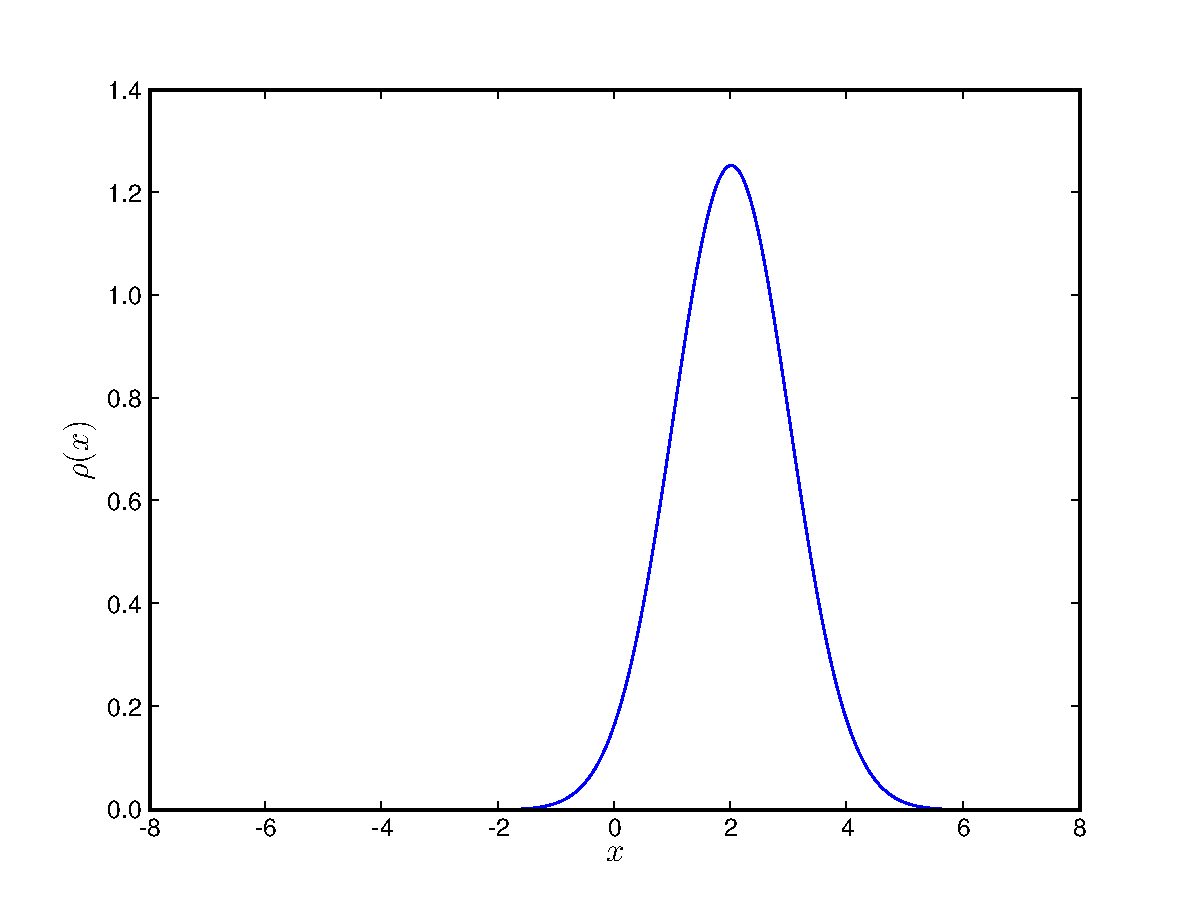
\includegraphics[width=0.8\textwidth]{Prob2.pdf}
\end{center}

\subsection*{Problem 3}
Let
\begin{equation*}
\Psi(x)= 
\begin{cases}
A(1+x) & -1\leq x\leq 0\,,\\
A(1-x) & 0\leq x\leq 1\,,\\
0      & x\notin [-1,1]\,.
\end{cases}
\end{equation*}
\textbf{a)} Determine $A$.

\textbf{b)} Determine $\langle x\rangle$, $\langle x^2\rangle$.

\textbf{c)} Determine $\sigma_x$.

\textbf{d)} Determine $\langle p\rangle$.

\subsubsection*{Solution}
\textbf{a)} We know that
\[
\rho(x)=\Psi(x)^*\Psi(x)=
\begin{cases}
A^2(1+2x+x^2) & -1\leq x\leq 0\,,\\
A^2(1-2x+x^2) & 0\leq x\leq 1\,,\\
0      & x\notin [-1,1]\,.
\end{cases}
\]
We must scale $A$ so that
\begin{align*}
\int_{-\infty}^\infty\rho(x)\,\d x
&=\int_{-1}^0 A^2(1+2x+x^2)\,\d x+\int_0^1 A^2(1-2x+x^2)\,\d x\\
&=\frac{2}{3}A^2=1\,.
\end{align*}
Therefore,
\[
A=\pm\sqrt{\frac{3}{2}}\,.
\]
\textbf{b)} Now we can find
\begin{align*}
\langle x\rangle
=\int_{-\infty}^\infty x\rho(x)\,\d x
&=\int_{-1}^0 A^2(x+2x^2+x^3)\,\d x+\int_0^1 A^2(x-2x^2+x^3)\,\d x\\
&=-\frac{1}{8}+\frac{1}{8}=0\,,
\end{align*}
and
\begin{align*}
\langle x^2\rangle
=\int_{-\infty}^\infty x^2\rho(x)\,\d x
&=\int_{-1}^0 A^2(x^2+2x^3+x^4)\,\d x+\int_0^1 A^2(x^2-2x^3+x^4)\,\d x\\
&=\frac{1}{20}+\frac{1}{20}=\frac{1}{10}\,.
\end{align*}
\textbf{c)} This gives us
\[
\sigma_x=\sqrt{\langle x^2\rangle-\langle
x\rangle^2}=\sqrt{\frac{1}{10}}=0.316\,.
\]
\textbf{d)} The equation for $\langle p\rangle$ is
\[
\langle p\rangle=m\frac{\d\langle x\rangle}{\d t}
=\int_{-\infty}^\infty\Psi^*p\Psi\,\d x\,,
\]
where $p\Psi=\frac{\hbar}{i}\frac{\partial}{\partial x}\Psi$, and
\[
\frac{\partial}{\partial x}\Psi=
\begin{cases}
A & -1\leq x\leq 0\,,\\
-A & 0\leq x\leq 1\,,\\
0      & x\notin [-1,1]\,.
\end{cases}\,.
\]
Therefore,
\[
\langle p\rangle=\int_{-\infty}^\infty\Psi^*p\Psi\,\d x
=\frac{\hbar}{i}\left[\int_{-1}^0 A^2(1+x)\,\d x
+\int_0^1 -A^2(1-x)\,\d x\right]=0\,.
\]
\subsection*{Problem 4}
The state of a quantum system is given by
\[
\Psi(x,t)=\alpha\e^{-\Lambda}\,,
\]
where
\[
\Lambda=\beta\hbar^{-1}(m x^2+i\gamma t)\,,
\]
and in which $\alpha\,,\beta$, and $\gamma$ are constants.

\textbf{a)} Find the potential energy $V(x)$ of this system.

\textbf{b)} Calculate the expected values of $x$, $x^2$, $p$, and $p^2$.

\textbf{c)} Calculate $\sigma_x$ and $\sigma_p$.  Are these consistent with the
Heisenberg principle?

\textbf{d)} What is $\alpha$?

\subsubsection*{Solution}
\textbf{a)} Schrodinger's equation with potential energy is
\[
\left(-\frac{\hbar^2}{2m}\frac{\partial^2}{\partial
x^2}+V(x)+\frac{\hbar}{i}\frac{\partial}{\partial t}\right)\Psi=0\,.
\]
Isolating $V(x)$,
\[
V(x)\Psi
=\frac{\hbar^2}{2m}\frac{\partial^2}{\partial x^2}\Psi
-\frac{\hbar}{i}\frac{\partial}{\partial t}\Psi\,.
\]
We can take the partial derivatives of $\Psi$,
\[
\frac{\partial^2}{\partial x^2}\Psi=-2\frac{\beta m}{\hbar}\Psi
+4\frac{\beta^2m^2x^2}{\hbar^2}\Psi\,,
\]
and
\[
\frac{\partial}{\partial t}\Psi=-\frac{i\beta\gamma}{\hbar}\Psi\,.
\]
Therefore
\begin{align*}
V(x)&=\Psi^{-1}\left(\frac{\hbar^2}{2m}\left(
-2\frac{\beta m}{\hbar}\Psi+4\frac{\beta^2m^2x^2}{\hbar^2}\Psi\right)
-\frac{\hbar}{i}\left(-\frac{i\beta\gamma}{\hbar}\Psi\right)\right)\\
&=\beta(-h+2\beta m x^2)-\beta\gamma\\
&=\beta(-h+2\beta m x^2+\gamma)\,.
\end{align*}
\textbf{b)} Assuming $\alpha$, $\beta$, $\gamma$ are real, the complex
conjugate of $\Psi$ is
\[
\Psi^*=\alpha\e^{-\frac{\beta}{\hbar}(m x^2-i\gamma t)}\,,
\]
and the probability density function is
\begin{align*}
\rho(x)&=\Psi^*\Psi=\alpha^2\e^{\frac{\beta}{\hbar}(m x^2-i\gamma t)
-\frac{\beta}{\hbar}(m x^2+i\gamma t)}\\
&=\alpha^2\e^{-2\frac{\beta}{\hbar}m x^2}\,.
\end{align*}
We need to normalize this so that
\[
\int_{-\infty}^\infty\alpha^2\e^{-2\frac{\beta}{\hbar}m x^2}
=\alpha^2\sqrt{\frac{\hbar\pi}{2\beta m}}=1\,.
\]
This implies that
\[
\alpha=\pm\left(\frac{2\beta m}{\hbar\pi}\right)^{\frac{1}{4}}\,.
\]
Now we can find (via Mathematica),
\[
\langle x\rangle=\int_{-\infty}^\infty x\rho(x)\,\d x
=\alpha^2\int_{-\infty}^\infty x\e^{-2\frac{\beta}{\hbar}m x^2}\,\d x=0\,,
\]
and
\[
\langle x^2\rangle=\int_{-\infty}^\infty x^2\rho(x)\,\d x
=\alpha^2\int_{-\infty}^\infty x\e^{-2\frac{\beta}{\hbar}m x^2}\,\d x
=\frac{\cancel{\alpha^2}\hbar}{4\beta m}\cancel{\sqrt{\frac{\hbar\pi}{2\beta
m}}}=\frac{\hbar}{4\beta m}\,.
\]
Also the expected value of momentum is
\[
\langle p\rangle=\int_{-\infty}^\infty\Psi^*p\Psi\,\d x\,,
\]
where
\[
p\Psi=\frac{\hbar}{i}\frac{\partial}{\partial x}\Psi
=\frac{\hbar}{i}\left(-\frac{2\beta m x}{\hbar}\right)\Psi
=2i\beta m x\Psi\,.
\]
Therefore
\[
\langle p\rangle=2i\beta m\int_{-\infty}^\infty x\Psi^*\Psi\,\d x=0\,.
\]
We can also calculate
\[
\langle p^2\rangle=\int_{-\infty}^\infty\Psi^*p^2\Psi\,\d x\,,
\]
where
\[
p^2\Psi=-\hbar^2\frac{\partial^2}{\partial x^2}\Psi
=-\hbar^2\left(-\frac{2\beta m}{\hbar}+\frac{4\beta m^2 x^2}{\hbar^2}\right)\Psi
=(2\beta\hbar m-4\beta m^2 x^2)\Psi\,.
\]
Therefore
\begin{align*}
\langle p^2\rangle&=\int_{-\infty}^\infty(2\beta\hbar m-4\beta^2 m^2 x^2)
\Psi^*\Psi\,\d x\\
&=2\beta\hbar m\underbrace{\int_{-\infty}^\infty\rho(x)\,\d x}_{1}
-4\beta^2 m^2\underbrace{\int_{-\infty}^\infty x^2\rho(x)\,\d x}_
{\langle x^2\rangle}\\
&=2\beta\hbar m-4\beta^2m^2\left(\frac{\hbar}{4\beta m}\right)\\
&=2\beta\hbar m-\beta m\hbar\\
&=\beta\hbar m\,.
\end{align*}
\textbf{c)} Now we can calculate the standard deviations,
\[
\sigma_x=\sqrt{\langle x^2\rangle-\langle x\rangle^2}
=\frac{1}{2}\sqrt{\frac{\hbar}{\beta m}}\,,
\]
and
\[
\sigma_p=\sqrt{\langle p^2\rangle-\langle p\rangle^2}
=\sqrt{\beta\hbar m}\,.
\]
These are consistent with the Heisenberg principle because
\[
\sigma_x\sigma_p=\frac{1}{2}\sqrt{\frac{\hbar}{\beta m}}\sqrt{\beta\hbar m}
=\frac{1}{2}\hbar\geq\frac{1}{2}\hbar\,.
\]
\textbf{d)} From earlier, we calculated that in order to normalize the
probability density function correctly,
\[
\alpha=\pm\left(\frac{2\beta m}{\hbar\pi}\right)^{\frac{1}{4}}\,.
\]
\end{document}

